%%%%%%%%%%%%%%%%%%%%%%%%%%%%%%%%%%%%%%%%%%%%%%%%%%%%%%%%%%%%%%%%%%%%%%%%%%%%%%%
% Titel:   Evaluation
% Autor:   Nicola K�ser
%%%%%%%%%%%%%%%%%%%%%%%%%%%%%%%%%%%%%%%%%%%%%%%%%%%%%%%%%%%%%%%%%%%%%%%%%%%%%%%
\chapter{Evaluation}\label{ch:evaluation}
Mit Hilfe der Liste konnte entschieden werden, welche Sensoren f�r die Evaluation bestellt werden. Einerseits wurden diverse Infrarot-Sensoren ausgew�hlt, anderseits auch Ultraschall-Module. Ein Laser-Sensor der in einer Eurobot-Thesis verwendet wurde, wurde auch noch dazu genommen. So konnte ein Einblick in alle erl�uterten  geeigneten Methoden gewonnen werden und die Vor- und Nachteile abgewogen werden.
%
	\section{GP2D120 und GP2Y0A02YK}\label{s:gp2d120_und_gp2y0a02yk}
	Die Infrarot-Sensoren GP2D120 und GP2Y0A02YK von Sharp basieren auf dem Triangulationsprinzip. Es sind Nachfolgemodelle der Typen wie die fr�heren Teams sie verwendeten.
	\begin{figure}[H]%H htbp
		\centering
		%%%%%%%%%%%%%%%%%%%%%%%%%%%%%%%%%%%%%%%%%%%%%%%%%%%%%%%%%%%%%%%%%%%%%%%%%%%%%%%
% Titel:   Diagramm: GP2D120
% Autor:   Nicola K�ser
%%%%%%%%%%%%%%%%%%%%%%%%%%%%%%%%%%%%%%%%%%%%%%%%%%%%%%%%%%%%%%%%%%%%%%%%%%%%%%%
\begin{tikzpicture}
	\begin{axis}[
		height=9cm, width=13cm,
		xlabel=Distanz/m, ylabel=U/V,
		grid=major,
		legend style={cells={anchor=west}}]
	%
	%\addplot[color=blue,mark=*] coordinates {
	\addplot coordinates {
		( 10, 2.32)
		( 12, 2.7 )
		( 15, 2.73)
		( 18, 2.6 )
		( 20, 2.52)
		( 30, 1.94)
		( 40, 1.48)
		( 50, 1.18)
		( 60, 0.98)
		( 80, 0.73)
		(100, 0.59)
		(140, 0.37)
	};
	\addlegendentry{Holz}
	%
	%\addplot[color=red,mark=square*] coordinates {
	\addplot coordinates {
		( 10, 2.73)
		( 12, 2.8 )
		( 15, 2.57)
		( 18, 2.3 )
		( 20, 2.2 )
		( 30, 1.73)
		( 40, 1.44)
		( 50, 1.14)
		( 60, 1.03)
		( 80, 0.79)
		(100, 0.66)
		(140, 0.5 )
	};
	\addlegendentry{Metall, gl�nzend}
	%
	%\addplot[color=teal,mark=triangle*] coordinates {
	\addplot coordinates {
		( 10, 2.52)
		( 12, 2.8 )
		( 15, 2.78)
		( 18, 2.62)
		( 20, 2.52)
		( 30, 1.96)
		( 40, 1.5 )
		( 50, 1.2 )
		( 60, 1   )
		( 80, 0.75)
		(100, 0.58)
		(140, 0.4 )
	};
	\addlegendentry{Metall, matt}
	%
	\end{axis}
\end{tikzpicture}
		\caption[Messungen mit dem IR-Sensor GP2D120]{Messungen mit dem Infrarotsensor GP2D120}
		\label{img:messung-gp2d120}
	\end{figure}
	%
	\begin{figure}[H]%H htbp
		\centering
		\begin{tikzpicture}
	\begin{axis}[
		height=9cm, width=13cm,
		xlabel=Distanz/m, ylabel=U/V,
		grid=major,
		legend style={cells={anchor=west}}]
	%
	%\addplot[color=blue,mark=*] coordinates {
	\addplot coordinates {
		( 1  , 2.05)
		( 1.5, 1.86)
		( 2  , 2.65)
		( 2.5, 3.06)
		( 2.7, 3.06)
		( 3  , 2.96)
		( 3.5, 2.82)
		( 4  , 2.54)
		( 5  , 2.13)
		( 6  , 1.85)
		( 7  , 1.62)
		( 8  , 1.44)
		(10  , 1.14)
		(15  , 0.77)
		(20  , 0.57)
		(30  , 0.34)
		(40  , 0.25)
	};
	\addlegendentry{Holz}
	%
	%\addplot[color=red,mark=square*] coordinates {
	\addplot coordinates {
		( 1  , 2.76 )
		( 1.5, 2.64 )
		( 2  , 2.56 )
		( 2.5, 2.57 )
		( 2.7, 2.54 )
		( 3  , 2.44 )
		( 3.5, 2.327)
		( 4  , 2.11 )
		( 5  , 1.84 )
		( 6  , 1.56 )
		( 7  , 1.39 )
		( 8  , 1.28 )
		(10  , 1.05 )
		(15  , 0.74 )
		(20  , 0.57 )
		(30  , 0.44 )
		(40  , 0.34 )
	};
	\addlegendentry{Metall, gl�nzend}
	%
	%\addplot[color=teal,mark=triangle*] coordinates {
	\addplot coordinates {
		( 1  , 2.69)
		( 1.5, 2.22)
		( 2  , 2.67)
		( 2.5, 3.02)
		( 2.7, 3.06)
		( 3  , 3.01)
		( 3.5, 2.83)
		( 4  , 2.51)
		( 5  , 2.13)
		( 6  , 1.85)
		( 7  , 1.63)
		( 8  , 1.47)
		(10  , 1.2 )
		(15  , 0.81)
		(20  , 0.61)
		(30  , 0.37)
		(40  , 0.27)
	};
	\addlegendentry{Metall, matt}
	%
	\end{axis}
\end{tikzpicture}
		\caption[Messungen mit dem IR-Sensor GP2Y0A02YK]{Messungen mit dem Infrarotsensor GP2Y0A02YK}
		\label{img:messung-gp2y0a02yk}
	\end{figure}
	%
	Die im vorherigen Kapitel beschriebenen Probleme wie Aussetzer und Messfehler konnten nicht reproduziert werden. Es gab einige Abweichungen wegen spiegelnder Oberfl�che der Objekte, dieses Ph�nomen ist aber gut nachvollziehbar. Im Diagramm ist jedoch zu erkennen, dass auch bei diesen Sensor-Versionen die in der Thesis beschriebene Problematik der zweideutigen Messresultate \cite{lit:gegnerischer_roboter} besteht.
	\begin{figure}[H]
	\centering
	\begin{minipage}[t]{.49\textwidth}
		\centering
		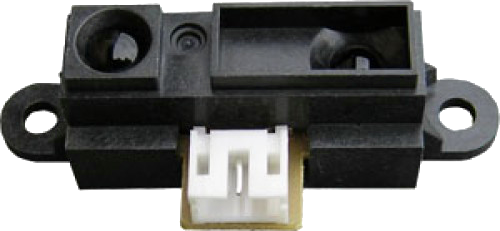
\includegraphics[scale=.2]{content/image/gp2d120}
		\captionof{figure}[GP2D120]{GP2D120 \cite{pic:sharp}}
		\label{pic:gp2d120}
	\end{minipage}
	\begin{minipage}[t]{.49\textwidth}
		\centering
		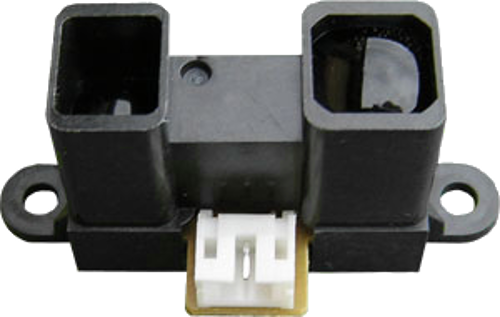
\includegraphics[scale=.2]{content/image/gp2y0a02yk}
		\captionof{figure}[GP2Y0A02YK]{GP2Y0A02YK \cite{pic:sharp}}
		\label{pic:gp2y0a02yk}
	\end{minipage}
	\end{figure}
	%
	\section{IS471F}\label{s:is471f}
	Auch von Sharp, ist der Sensor IS471F. Dabei handelt es sich um ein Bauteil, das in einer einfachen Schaltung als Distanzschalter funktioniert.
	\image{content/image/is471f}{scale=.5}[Einfache Beispielschaltung mit Sensor IS471F \cite{pic:is471f}][Einfache Beispielschaltung mit Sensor IS471F][pic:is471f]
	Die im Sensor integrierte Schaltung steuert externe Infrarot-LEDs an. Ist das so modulierte Licht f�r den Sensor sichtbar, wo liefert dieser einen definierten Pegel, andernfalls den invertierten Pegel. Dies funktioniert nicht nur bei direkter Bestrahlung, wie bei Lichtschranken, sondern auch bei Reflektiertem Licht. F�r die Naherkennung k�nnte also �ber die Lichtst�rke die Schaltdistanz eingestellt werden.
	\begin{figure}[H]%H htbp
		\centering
		%%%%%%%%%%%%%%%%%%%%%%%%%%%%%%%%%%%%%%%%%%%%%%%%%%%%%%%%%%%%%%%%%%%%%%%%%%%%%%%
% Titel:   Diagramm: IS471F
% Autor:   Nicola K�ser
%%%%%%%%%%%%%%%%%%%%%%%%%%%%%%%%%%%%%%%%%%%%%%%%%%%%%%%%%%%%%%%%%%%%%%%%%%%%%%%
\begin{tikzpicture}
	\begin{axis}[
		ybar,
		bar width=5mm,
		height=4.095cm, width=9cm,
		ylabel=Distanz/m,
		ymajorgrids=true,
		enlargelimits=0.5,
		legend style={
			cells={anchor=west},
			legend pos=outer north east
		},
		xtick=data,
		nodes near coords,
		nodes near coords align={vertical},
		symbolic x coords={Normale LED, Helle LED}]
	%
	\addplot coordinates{(Normale LED, 17) (Helle LED, 35)};
	\addplot coordinates{(Normale LED, 30) (Helle LED, 47)};
	\addplot coordinates{(Normale LED, 40) (Helle LED, 52)};
	\addplot coordinates{(Normale LED, 27) (Helle LED, 37)};
	\addplot coordinates{(Normale LED,  6) (Helle LED,  9)};
	\legend{Holz, {Metall, matt}, {Metall, gl�nzend}, {Metall, eloxiert schwarz}, {Plastik, matt schwarz}}
	%
	\end{axis}
\end{tikzpicture}
		\caption[Messungen mit dem IR-Sensor IS471F]{Messungen mit dem Infrarotsensor IS471F}
		\label{img:messung-is471f}
	\end{figure}
	Auch hier sind Abweichungen bez�glich des Materials/Oberfl�che festzustellen. Es ist ausserdem gut zu erkennen, dass die Helligkeit der LEDs Einfluss auf die Schaltdistanz hat. Mit einer Hellen LED (SFH 485-2) konnte auch die gemessene Distanz zu einer Holzoberfl�che �ber \SI{20}{\centi\meter} gehoben werden.
	%
	\section{SRF-Module von Devantech}\label{s:srf-module_von_devantech}
	\begin{figure}[H]
	\centering
	\begin{minipage}[t]{.3\textwidth}
		\centering
		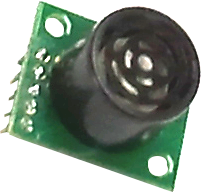
\includegraphics[scale=.2]{content/image/srf02}
		\captionof{figure}{SRF02}
		\label{pic:srf02}
	\end{minipage}
	\begin{minipage}[t]{.3\textwidth}
		\centering
		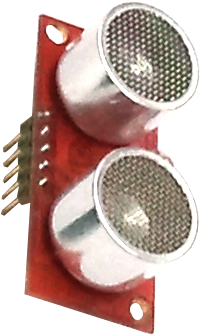
\includegraphics[scale=.2]{content/image/srf08}
		\captionof{figure}{SRF08}
		\label{pic:srf08}
	\end{minipage}
	\begin{minipage}[t]{.3\textwidth}
		\centering
		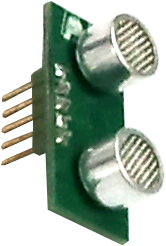
\includegraphics[scale=.2]{content/image/srf10}
		\captionof{figure}{SRF10}
		\label{pic:srf10}
	\end{minipage}
	\end{figure}
	%
	Devantech\footnote{\url{http://www.devantech.co.uk/}} entwickelt diverse elektronische Module, darunter befindet sich auch eine Reihe von Ultraschall-Modulen zur Distanzmessung.
	F�r die Evaluation wurden drei Typen im \SI{40}{\kilo\hertz}-Bereich ausgew�hlt. Diese lassen sich alle mit \iic\ ansteuern und verwenden die gleiche Kommunikation, die Ansteuerung aller Sensoren ist also mit der gleichen Software m�glich. Ausgelesen k�nnen Werte in Zentimeter, Inch und Milisekunden.
	%
		\subsection{SRF02}
		Der Typ SRF02 weist die kleinste Bauform auf. Das Modul besteht nicht aus separatem Ultraschallsender und -empf�nger, sondern die beiden Elemente sind in einem kombiniert. Der Erfassungsbereich wird vom Hersteller mit 55� angegeben \cite{url:spec_srf02}. Bei diesem Modul w�re zus�tzlich zu \iic\ eine Ansteuerung mit RS-232 m�glich, welche jedoch nicht getestet wurde.
		\begin{figure}[H]%H htbp
			\centering
			%%%%%%%%%%%%%%%%%%%%%%%%%%%%%%%%%%%%%%%%%%%%%%%%%%%%%%%%%%%%%%%%%%%%%%%%%%%%%%%
% Titel:   Diagramm: SRF02
% Autor:   Nicola Käser
%%%%%%%%%%%%%%%%%%%%%%%%%%%%%%%%%%%%%%%%%%%%%%%%%%%%%%%%%%%%%%%%%%%%%%%%%%%%%%%
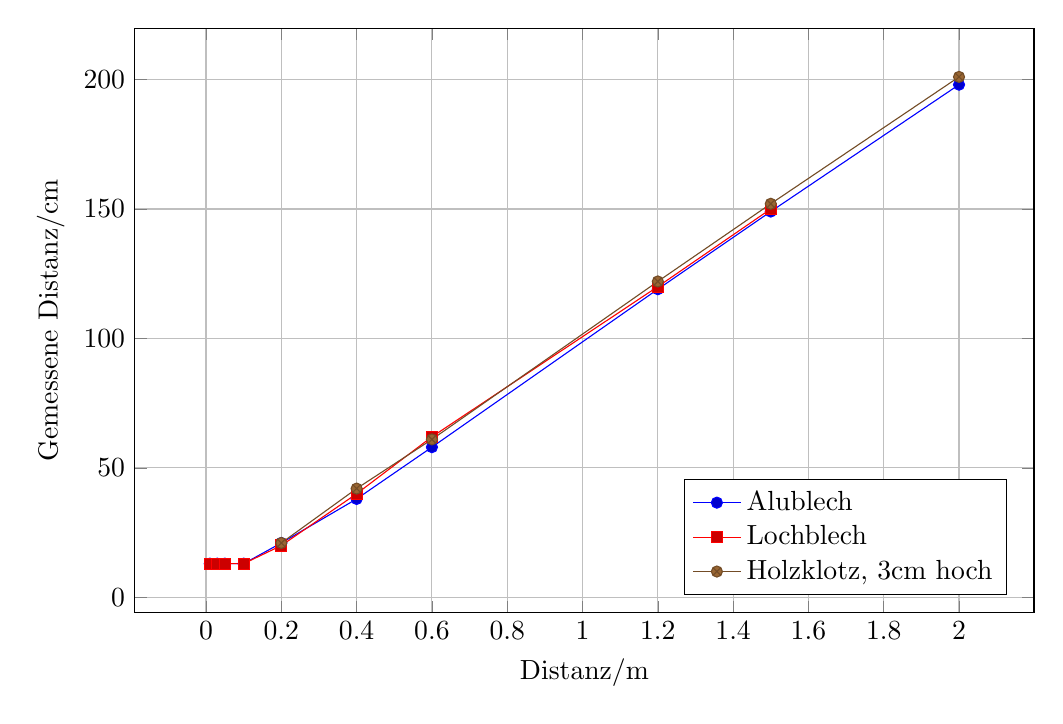
\begin{tikzpicture}
	\begin{axis}[
		height=9cm, width=13cm,
		xlabel=Distanz/m, ylabel=Gemessene Distanz/cm,
		grid=major,
		legend style={
			cells={anchor=west},
			legend pos=south east
		}]
	%
	%\addplot[color=blue,mark=*] coordinates {
	\addplot coordinates {
		(0.01,  13)
		(0.03,  13)
		(0.05,  13)
		(0.10,  13)
		(0.20,  21)
		(0.40,  38)
		(0.60,  58)
		(1.20, 119)
		(1.50, 149)
		(2.00, 198)
	};
	\addlegendentry{Alublech}
	%
	%\addplot[color=red,mark=square*] coordinates {
	\addplot coordinates {
		(0.01,  13)
		(0.03,  13)
		(0.05,  13)
		(0.10,  13)
		(0.20,  20)
		(0.40,  40)
		(0.60,  62)
		(1.20, 120)
		(1.50, 150)
		%(2.00, 150)
	};
	\addlegendentry{Lochblech}
	%
	%\addplot[color=teal,mark=triangle*] coordinates {
	\addplot coordinates {
		(0.20,  21)
		(0.40,  42)
		(0.60,  61)
		(1.20, 122)
		(1.50, 152)
		(2.00, 201)
	};
	\addlegendentry{Holzklotz, 3cm hoch}
	%
	\end{axis}
\end{tikzpicture}
			\caption[Messungen mit dem Ultraschallsensor SRF02]{Messungen mit dem Ultraschallsensor SRF02}
			\label{img:messung-srf02}
		\end{figure}
		%
		Im Diagramm sind kleine Unterschiede, abh�ngig von der Objektgeometrie, erkennbar. Im Allgemeinen wird die Distanz jedoch relativ zuverl�ssig gemessen. Gut erkennbar ist auch, dass zu kleine Distanzen (nicht im Messbereich des Sensors) trotzdem noch erkannt werden und den Mimimalwert anzeigen. Beim Messen gab es ein paar Ausreisser die erneut gemessen werden mussten.
		%
		\subsection{SRF08}
		Dieses Modul ist das gr�sste der evaluierten Modulen von Devantech. Auch hier wird der Erfassungsbereich mit 55� angegeben \cite{url:spec_srf08}.
		Zus�tzlich zum Ultraschallsender und -empf�nger befindet sich auch eine Fotodiode auf dem Print. Diese k�nnte auch per \iic\ ausgelesen werden, wurde jedoch nicht getestet.
		\begin{figure}[H]%H htbp
			\centering
			%%%%%%%%%%%%%%%%%%%%%%%%%%%%%%%%%%%%%%%%%%%%%%%%%%%%%%%%%%%%%%%%%%%%%%%%%%%%%%%
% Titel:   Diagramm: SRF08
% Autor:   Nicola Käser
%%%%%%%%%%%%%%%%%%%%%%%%%%%%%%%%%%%%%%%%%%%%%%%%%%%%%%%%%%%%%%%%%%%%%%%%%%%%%%%
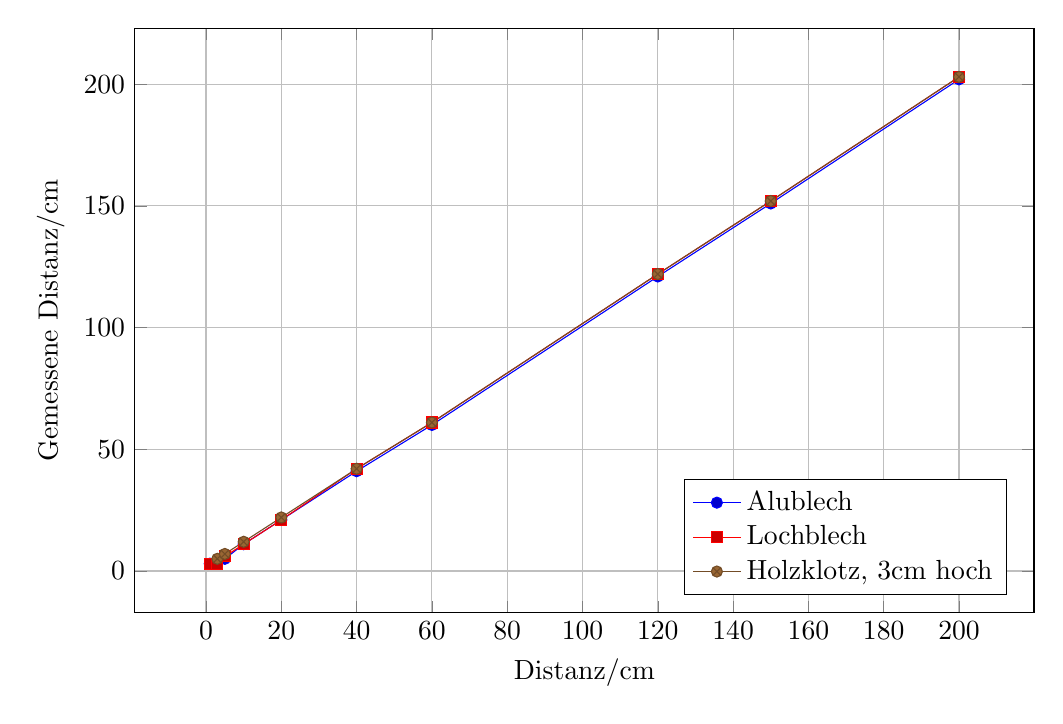
\begin{tikzpicture}
	\begin{axis}[
		height=9cm, width=13cm,
		xlabel=Distanz/cm, ylabel=Gemessene Distanz/cm,
		grid=major,
		legend style={
			cells={anchor=west},
			legend pos=south east
		}]
	%
	%\addplot[color=blue,mark=*] coordinates {
	\addplot coordinates {
		(  1,   3)
		(  3,   4)
		(  5,   5)
		( 10,  11)
		( 20,  21)
		( 40,  41)
		( 60,  60)
		(120, 121)
		(150, 151)
		(200, 202)
	};
	\addlegendentry{Alublech}
	%
	%\addplot[color=red,mark=square*] coordinates {
	\addplot coordinates {
		(  1,   3)
		(  3,   3)
		(  5,   6)
		( 10,  11)
		( 20,  21)
		( 40,  42)
		( 60,  61)
		(120, 122)
		(150, 152)
		(200, 203)
	};
	\addlegendentry{Lochblech}
	%
	%\addplot[color=teal,mark=triangle*] coordinates {
	\addplot coordinates {
		(  3,   5)
		(  5,   7)
		( 10,  12)
		( 20,  22)
		( 40,  42)
		( 60,  61)
		(120, 122)
		(150, 152)
		(200, 203)
	};
	\addlegendentry{Holzklotz, 3cm hoch}
	%
	\end{axis}
\end{tikzpicture}
			\caption[Messungen mit dem Ultraschallsensor SRF08]{Messungen mit dem Ultraschallsensor SRF08}
			\label{img:messung-srf08}
		\end{figure}
		Dieser Sensor lieferte die besten Messergebnisse der Devantech-Ultraschallmodule. Dies ist auch im Diagramm erkennbar, es waren nur geringe Abweichungen feststellbar.
		%
		\subsection{SRF10}
		Beim Typ SRF10 ist die Bauform gleich wie beim SRF08, jedoch ist der Ultraschallsender und -empf�nger kleiner. Der Erfassungsbereich ist gr�sser als bei den anderen beiden Modulen, laut Hersteller 75� \cite{url:spec_srf10}.
		\begin{figure}[H]%H htbp
			\centering
			%%%%%%%%%%%%%%%%%%%%%%%%%%%%%%%%%%%%%%%%%%%%%%%%%%%%%%%%%%%%%%%%%%%%%%%%%%%%%%%
% Titel:   Diagramm: SRF10
% Autor:   Nicola Käser
%%%%%%%%%%%%%%%%%%%%%%%%%%%%%%%%%%%%%%%%%%%%%%%%%%%%%%%%%%%%%%%%%%%%%%%%%%%%%%%
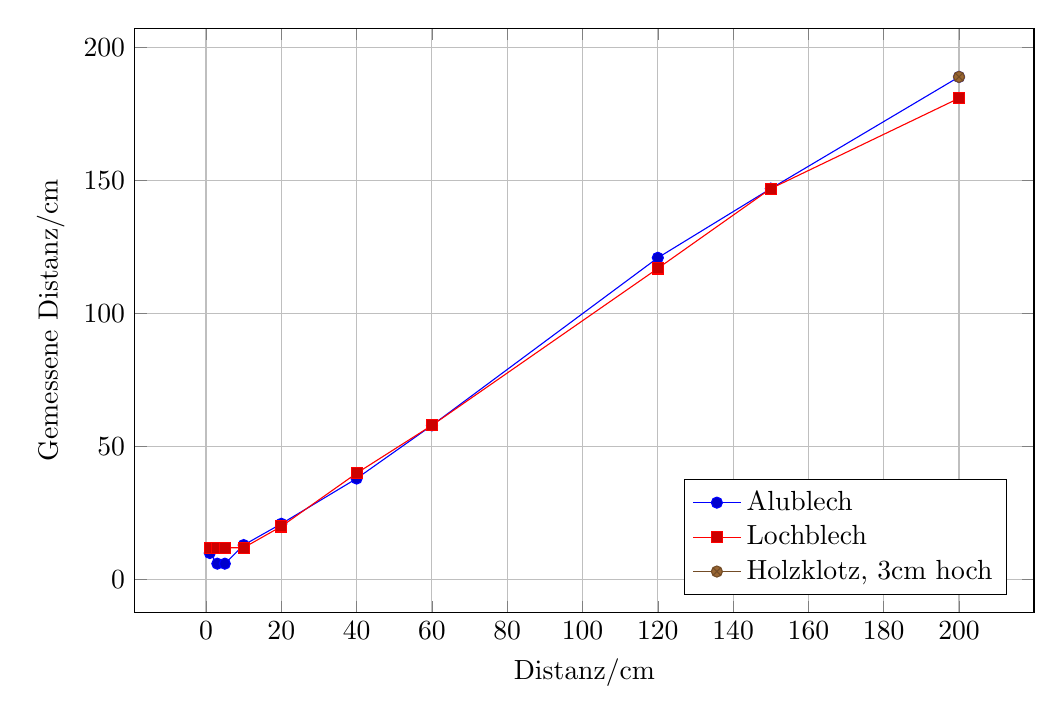
\begin{tikzpicture}
	\begin{axis}[
		height=9cm, width=13cm,
		xlabel=Distanz/cm, ylabel=Gemessene Distanz/cm,
		grid=major,
		legend style={
			cells={anchor=west},
			legend pos=south east
		}]
	%
	%\addplot[color=blue,mark=*] coordinates {
	\addplot coordinates {
		(  1,  10)
		(  3,   6)
		(  5,   6)
		( 10,  13)
		( 20,  21)
		( 40,  38)
		( 60,  58)
		(120, 121)
		(150, 147)
		(200, 189)
	};
	\addlegendentry{Alublech}
	%
	%\addplot[color=red,mark=square*] coordinates {
	\addplot coordinates {
		(  1,  12)
		(  3,  12)
		(  5,  12)
		( 10,  12)
		( 20,  20)
		( 40,  40)
		( 60,  58)
		(120, 117)
		(150, 147)
		(200, 181)
	};
	\addlegendentry{Lochblech}
	%
	%\addplot[color=teal,mark=triangle*] coordinates {
	\addplot coordinates {
		(200, 189)
	};
	\addlegendentry{Holzklotz, 3cm hoch}
	%
	\end{axis}
\end{tikzpicture}
			\caption[Messungen mit dem Ultraschallsensor SRF10]{Messungen mit dem Ultraschallsensor SRF10}
			\label{img:messung-srf10}
		\end{figure}
		Dass bei diesem Modul der Erfassungsbereich gr�sser ist, war beim Messen gut feststellbar. Es musste �fters eine Messung wiederholt werden, da die Distanz zur Seitenwand oder zu anderen Objekten seitlich in der N�he gemessen wurde statt die Distanz geradeaus zum Messobjekt. Wie im Diagramm erkennbar ist, wurde der \SI{3}{\centi\meter}-Holzklotz nur in \SI{2}{\meter} erkannt. Grund daf�r k�nnte die, im Gegensatz zu den anderen Modulen, h�here Positionierung sein, die aufgrund der vorher beschriebenen Messschwierigkeiten vorgenommen wurde.
		%
	\section{Lasersensor von Baumer}\label{s:lasersensor_von_baumer}
	Der Sensor OADM 13U7480/S35A von Baumer\footnote{\url{http://www.baumer.com/ch-de/}} wurde bereits vom letztj�hrigen Team evaluiert, und f�r den "`Gegnerischen Roboter"' verwendet \cite{lit:gegnerischer_roboter}. Aus diesem Grund wurde keine erneute vollst�ndige Evaluation, sonder lediglich eine Inbetriebnahme durchgef�hrt.
	\missingfigure{Bild von Sensor}
	Der Lasersensor liefert genaue Messergebnisse, diese sind jedoch nur punktuell. Aus diesem Grund wurde in der vorher genannten Thesisarbeit drei dieser Sensoren verwendet \cite{lit:gegnerischer_roboter}.
	%
	\section{Entscheidung}\label{s:entscheidung}
	Zur Entscheidungsfindung f�r den optimalen Sensortypen wurde eine Nutzwertanalyse gemacht:
	%%%%%%%%%%%%%%%%%%%%%%%%%%%%%%%%%%%%%%%%%%%%%%%%%%%%%%%%%%%%%%%%%%%%%%%%%%%%%%%
% Titel:   Nutzwertanalyse
% Autor:   Nicola K�ser
%%%%%%%%%%%%%%%%%%%%%%%%%%%%%%%%%%%%%%%%%%%%%%%%%%%%%%%%%%%%%%%%%%%%%%%%%%%%%%%
\begin{table}[H]
	% Lokale Commands (nur g�ltig bis \end{table})
	\newcommand{\R}[1]{\rotatebox{90}{#1}}  % 90� rotierte Zelle
	\newcommand{\T}[1]{\R{\textcolor{white}{\textbf{#1}}}}  % Titel, rotiert
	\newcommand{\mc}[1]{\multicolumn{2}{c|}{#1}}  % Zwei Zellen zusammengefasst
	\newcommand{\Tc}[1]{\mc{\T{#1}}}  % Titel, rotiert, zwei Zellen zusammengefasst
	\newcommand{\e}{\multicolumn{1}{c|}{\cellcolor{white}{~}}}  % Weisse Zelle ohne Linie links & oben
	\newcommand{\n}[2][c]{\begin{tabular}[#1]{@{}c@{}}#2\end{tabular}}  % Spezielle Zelle in der Umruch (\\) verwendet werden kann
	\definecolor{lightgreen}{HTML}{80FF80}
	\newcommand{\cA}[1]{\cellcolor{green}{#1}}  % Zellenfarbe 1
	\newcommand{\cB}[1]{\cellcolor{lightgreen}{#1}}  % Zellenfarbe 2
	%
	\centering
	% Schriftgr�sse etwas kleiner, damit gesammte Tabelle auf Seite passt
	\KOMAoptions{fontsize=10pt}
	\begin{tabular}{|l|c|c|c|c|c|c|c|c|c|c|c|c|c|c|c|}
	\cline{2-16}\rowcolor{bfhblue}
	\e               & \T{Gewichtung} & \Tc{A: GP2D120} & \Tc{B: GP2Y0A02YK} & \Tc{C: IS471F} & \Tc{D: SRF02} & \Tc{E: SRF08} & \Tc{F: SRF10} & \Tc{G: OADM} \\ \hline
	\textbf{Kriterien}      & \R{X} & \R{A} & \R{A*X } & \R{B} & \R{B*X } & \R{C} & \R{C*X } & \R{D} & \R{D*X } & \R{E} & \R{E*X } & \R{F} & \R{F*X } & \R{G} & \R{G*X } \\ \hline
	\n{Genau-\\igkeit}      & 9     & 7     & 63       & 8     & 72       & 2     & 18       & 8     & 72       & 9     & 81       & 8     & 72       & 10    & 90       \\ \hline
	\n{Zuverl�s-\\sigkeit}  & 10    & 5     & 50       & 4     & 40       & 8     & 80       & 6     & 60       & 8     & 80       & 4     & 40       & 8     & 80       \\ \hline
	\n{Geschwin-\\digkeit}  & 5     & 8     & 40       & 8     & 40       & 8     & 40       & 5     & 25       & 5     & 25       & 5     & 25       & 10    & 50       \\ \hline
	\n{Platz-\\bedarf}      & 7     & 7     & 49       & 6     & 42       & 9     & 63       & 8     & 56       & 6     & 42       & 8     & 56       & 1     & 7        \\ \hline
	\n{Energie-\\verbrauch} & 2     & 8     & 16       & 8     & 16       & 9     & 18       & 8     & 16       & 8     & 16       & 8     & 16       & 4     & 8        \\ \hline
	\n{Sicher-\\heit}       & 8     & 10    & 80       & 10    & 80       & 10    & 80       & 10    & 80       & 10    & 80       & 10    & 80       & 5     & 40       \\ \hline
	\n{Ansteu-\\erung}      & 3     & 5     & 15       & 5     & 15       & 6     & 18       & 6     & 18       & 6     & 18       & 6     & 18       & 5     & 15       \\ \hline
	\n{Kosten-\\aufwand}    & 4     & 7     & 28       & 6     & 24       & 10    & 40       & 7     & 28       & 6     & 24       & 6     & 24       & 2     & 8        \\ \hline\hline
	\textbf{Summe}          & 48    & 57    & 341      & 55    & 329      & 62    & \cB{357} & 58    & \cB{355} & 58    & \cA{366} & 55    & 331      & 45    & 298      \\ \hline
	\end{tabular}
	% Schriftgr�sse zur�cksetzten
	\KOMAoptions{fontsize=\defaultfontsize}
	\caption{Nutzwertanalyse zur Auswahl des optimalen Sensortyps}
	\label{tab:nutzwertanalyse}
\end{table}
	%
	Nach dieser Analyse ist ersichtlich, dass sich das Ultraschallsensor-Modul SRF08 von Devantech am Besten f�r die Naherkennung eignet. Auch hohe Wertung hat der Sensor IS471F von Sharp, sowie ein weiteres Ultraschall-Modul SRF02. Ich habe mich desshalb entschieden, f�r die Naherkennung das Modul SRF08 und zus�tzlich als zweite Absicherung den Sensor IS471F zu verwenden. So k�nnen die Nachteile beider Sensoren durch den anderen ausgeglichen werden.
	%